\documentclass[11pt]{article}
\usepackage{xcolor}
\usepackage{graphicx}
\usepackage{subfigure}
\usepackage[graphicx]{realboxes}
%\input{definitions}

\renewcommand{\baselinestretch}{1.2}
\setlength{\topmargin}{-0.25in}
\setlength{\oddsidemargin}{0.50in}
\setlength{\textwidth}{5.9in}
\setlength{\textheight}{8.5in}

\newcommand{\Answer}{\color{red}\textbf{Answer:} \color{black}}
\newcommand{\I}{{\bf I}}
\begin{document}
\begin{center}
{\bf Computer Vision I: Python Exercise / project \#1 } (total 10 points)\\
Due October 8, 2024, 2 pm\\

{\bf [Wang Keran] [2100017727]}
\end{center}

This is a small project designed to confirm certain characteristics of natural image statistics, as previously discussed in Chapter 2. Among the materials, you will find three distinct image sets:
\begin{enumerate}
 \item Set A consists of four natural images, including two captured in urban settings and two in countryside scenes.
 \item Set B comprises two man-made images, specifically paintings by Vincent van Gogh.
 \item Set C encompasses a random noise image.
\end{enumerate}


{\bf Python Library:} To complete the project, please install the required dependencies provided in the \textit{environment.yml} file (including cv2, PIL, numpy, scipy, matplotlib, tqdm). You are also welcome to utilize any libraries of your choice, \textbf{but please report them in your report (for autograder)!}
\color{red}
\textbf{Again, report any customized library in the report (do not go too crazy as this will add a significant burden to TAs).}
\color{black}

 {\bf What to hand in:} Please submit both a formal report and the accompanying code. For the report, kindly provide a PDF version. You may opt to compose a new report or complete the designated sections within this document, as can be started by simply loading the tex file to Overleaf. Your score will be based on the quality of \textbf{your results}, \textbf{the analysis} (diagnostics of issues and comparisons) of these results in your report, and your \textbf{code implementation}.

 {\bf Notice:} Hint code is provided, please \textbf{don't change} the name of the functions for automatic scoring, but feel free to add new functions.

\clearpage

\noindent{\bf Problem 1} (High kurtosis and scale invariance, 4 points). \emph{Please read through this question description before you start.} \emph{For this problem, please consider 3 sets: set A, set B, set C.} 

\noindent{For the sake of computational efficiency,}, convert the images to grayscale and subsequently rescale the intensity levels to fall within the range [0, 31], i.e. 32 grey levels. Please note that this rescaling operation is not necessary for the random image selected from set C. Then convolve the images with a gradient filter denoted as $\nabla_x I$, which signifies the intensity difference between two adjacent pixels along the horizontal axis. 
Accumulate the histograms by computing the averages over all images within each respective set. To illustrate, the process of accumulating the histogram for "set A" entails the aggregation of histograms from all four natural images found within "set A". Subsequently, complete the following steps for all sets.

\begin{enumerate}
\item Plot the histogram $H(z)$ for the difference against the horizontal axis $z \in [-31, +31]$. Then do a log-plot $\log H(z)$. [Some bins will be zero, you can assign $\epsilon$ for such bins in the log-plot]. 

\Answer See the Figure 1 and Figure 2
\begin{figure}[h]
    \centering
    \subfigure[Set A]{
        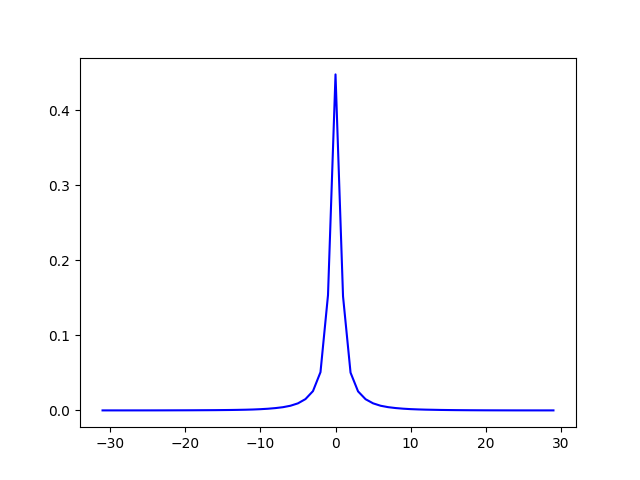
\includegraphics[scale=0.25]{pro1_result/downsampled_histogram/original_setA.png}
    }
    \subfigure[Set B]{
        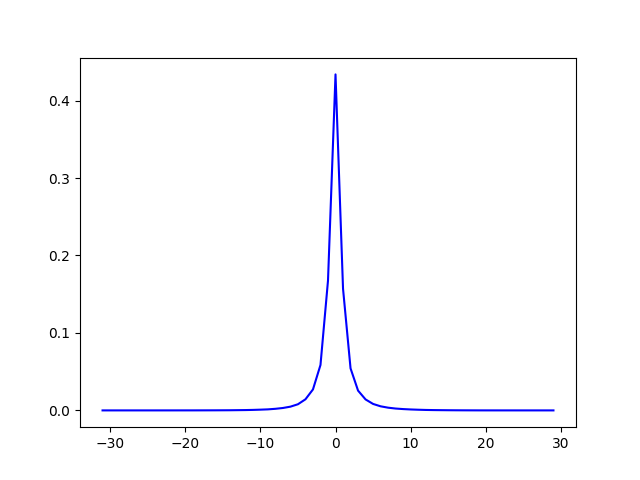
\includegraphics[scale=0.25]{pro1_result/downsampled_histogram/original_setB.png}
    }
    \subfigure[Set C]{
        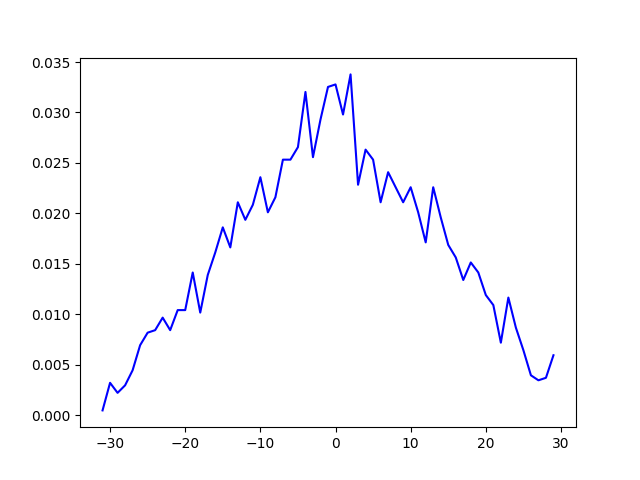
\includegraphics[scale=0.25]{pro1_result/downsampled_histogram/original_setC.png}
    }
    \caption{The Histograms $H(t)$}
\end{figure}
\begin{figure}[h]
    \centering
    \subfigure[Set A]{
        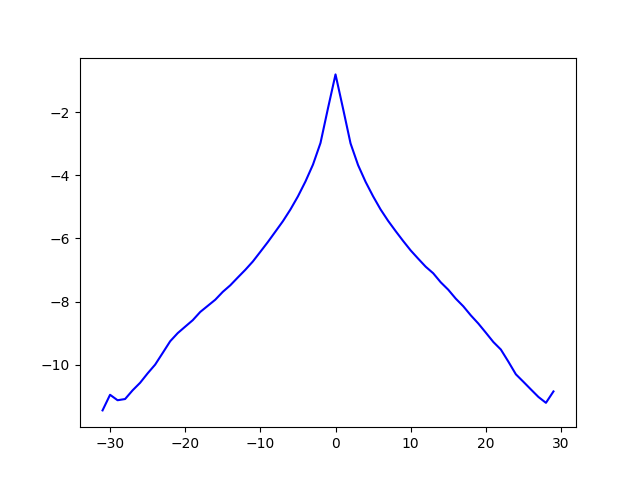
\includegraphics[scale=0.25]{pro1_result/log_histogram/setA.png}
    }
    \subfigure[Set B]{
        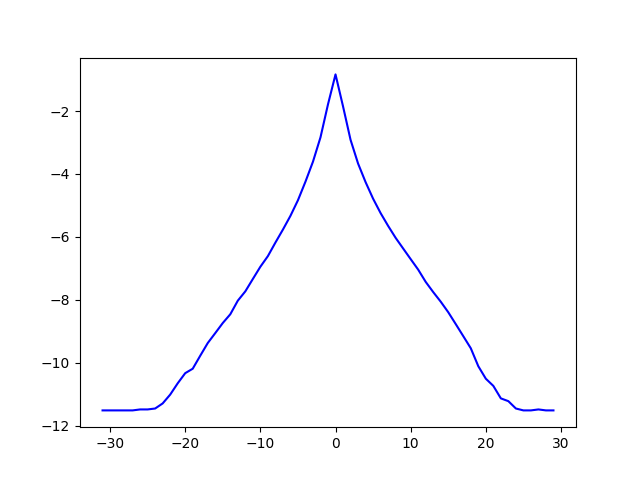
\includegraphics[scale=0.25]{pro1_result/log_histogram/setB.png}
    }
    \subfigure[Set C]{
        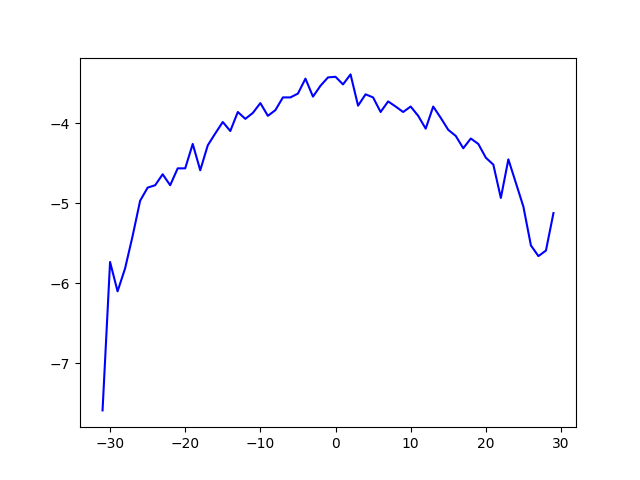
\includegraphics[scale=0.25]{pro1_result/log_histogram/setC.png}
    }
    \caption{The log-plot $\log H(t)$}
\end{figure}

\item Compute the mean, variance, and kurtosis for this histogram [Report the numeric numbers in your report].

\Answer See the Table 1

\begin{table}[h]
    \centering
    \begin{tabular}{|c|c|c|c|}
        \hline
        & mean & variance & kurtosis \\
        \hline
        set A & $-8.00\times 10^{-4}$ & 6.38 & 18.81 \\
        \hline
        set B & $5.97\times 10^{-4}$ & 4.39 & 14.58 \\
        \hline
        set C & $1.04\times 10^{-2}$ & 171.12 & 2.39 \\
        \hline
    \end{tabular}
    \caption{The mean, variance and kurtosis}
\end{table}


\item Fit this histogram to a Generalized Gaussian distribution $e^{|z/\sigma|^\gamma}$ and plot the fitted-curves super-imposed against the histogram. What is the value of $\gamma$ in the fitted generalized Gaussian?

\Answer See the Figure 3 and Tabel 2

the blue one is the original curve and the red one is the fitting curve
\begin{figure}[h]
    \centering
    \subfigure[Set A]{
        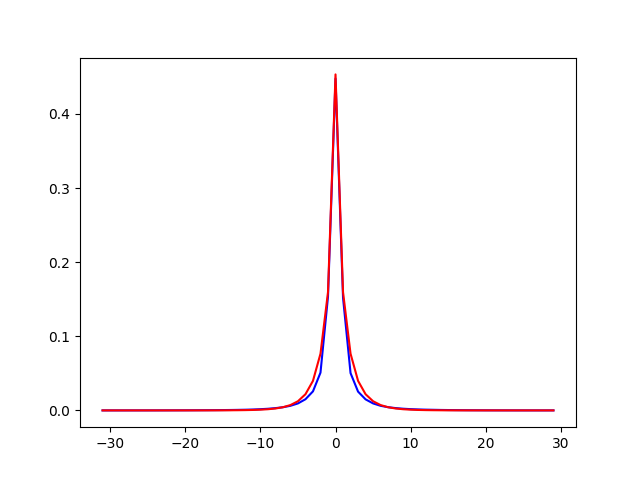
\includegraphics[scale=0.25]{pro1_result/histogram/setA.png}
    }
    \subfigure[Set B]{
        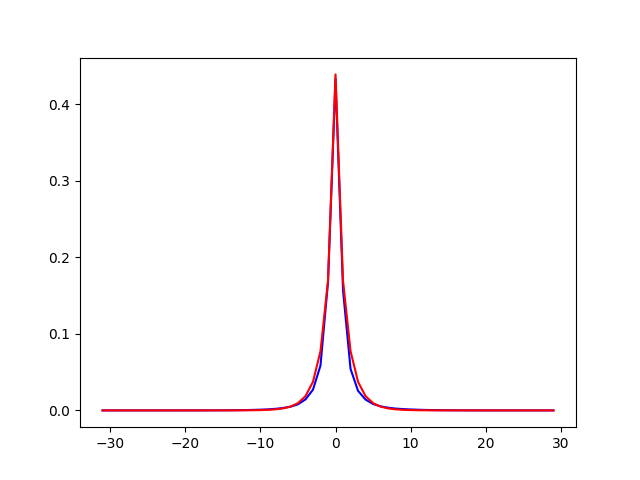
\includegraphics[scale=0.25]{pro1_result/histogram/setB.png}
    }
    \subfigure[Set C]{
        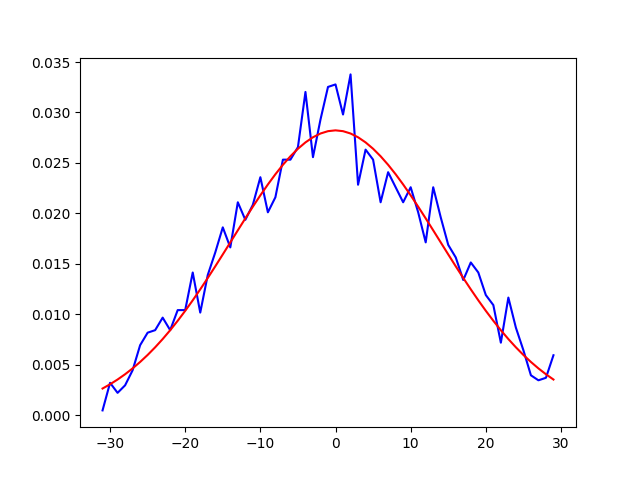
\includegraphics[scale=0.25]{pro1_result/histogram/setC.png}
    }
    \caption{The original curve and fitting curve}
\end{figure}
\begin{table}[h]
    \centering
    \begin{tabular}{|c|c|c|c|}
        \hline
         & set A & set B & set C \\
        \hline
        $\gamma$ & 0.770 & 0.866 & 1.954 \\
        \hline
    \end{tabular}
    \caption{The fittest $\gamma$ for set A,B,C}
\end{table}

\item Plot the Gaussian distribution using the mean and the variance in step (2), and super-impose this plot with the plots in step (1) above (i.e. plot the Gaussian and its log plot, this is easy to do in python with matplotlib).

\Answer See the Figure 4
\begin{figure}[h]
    \centering
    \subfigure[Set A]{
        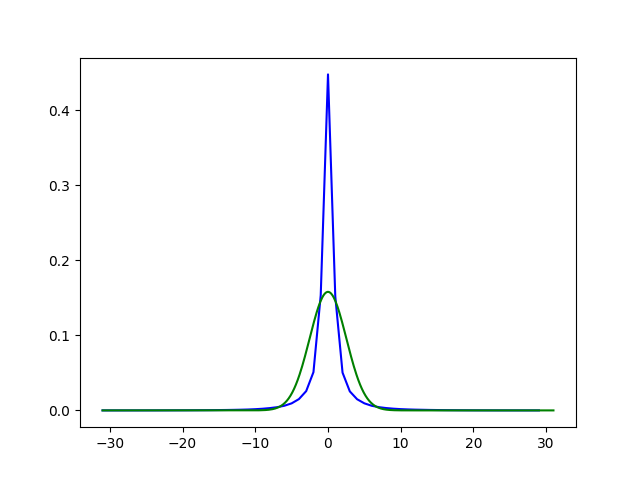
\includegraphics[scale=0.25]{pro1_result/histogram/setA_with Gaussian.png}
    }
    \subfigure[Set B]{
        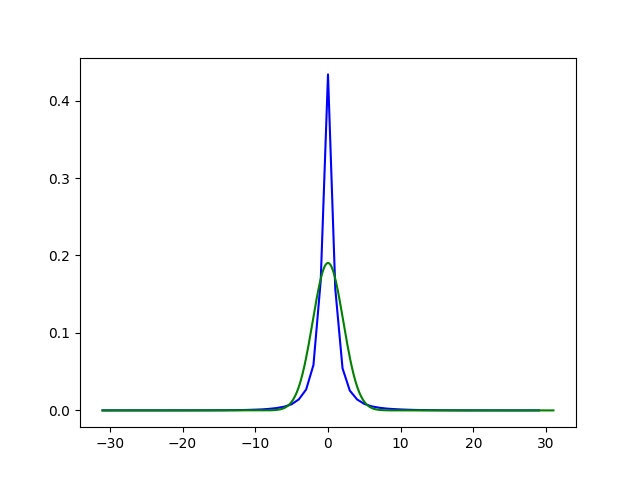
\includegraphics[scale=0.25]{pro1_result/histogram/setB_with Gaussian.png}
    }
    \subfigure[Set C]{
        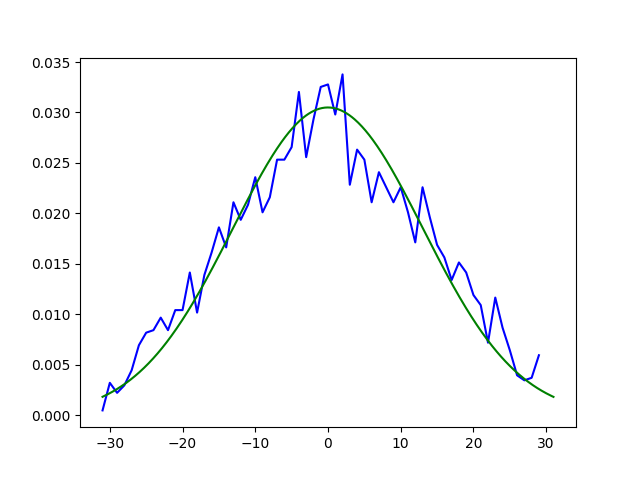
\includegraphics[scale=0.25]{pro1_result/histogram/setC_with Gaussian.png}
    }
    \caption{The original curve and Gaussian curve}
\end{figure}


\item Down-sample your images by a $2\times 2$ average (or simply sub-sample) the image. Plot the histogram and log histogram, and impose with the plots in step 1, to compare the difference. Repeat this down-sampling process 2-3 times. 

\Answer See the Figure 5 and Figure 6
\begin{figure}[h]
    \centering
    \subfigure[Set A]{
        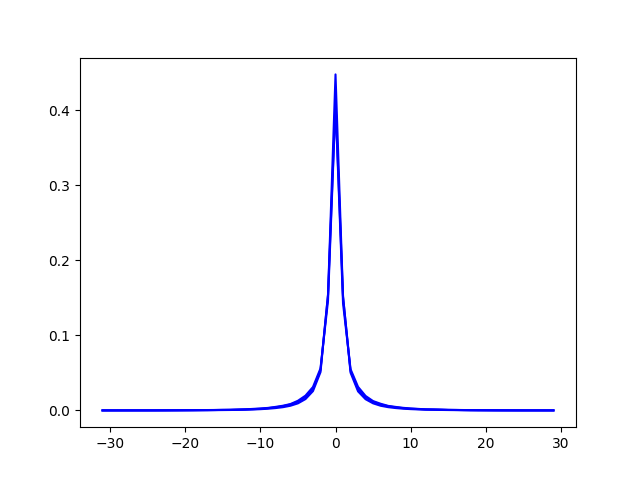
\includegraphics[scale=0.25]{pro1_result/downsampled_histogram/composed_setA.png}
    }
    \subfigure[Set B]{
        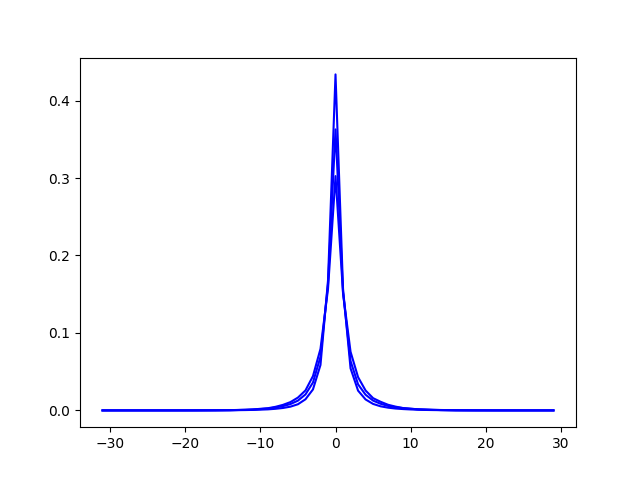
\includegraphics[scale=0.25]{pro1_result/downsampled_histogram/composed_setB.png}
    }
    \subfigure[Set C]{
        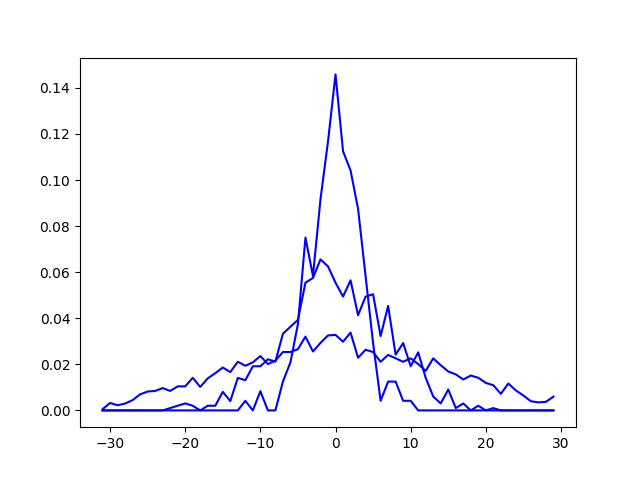
\includegraphics[scale=0.25]{pro1_result/downsampled_histogram/composed_setC.png}
    }
    \caption{Histograms and downsamples}
\end{figure}
\begin{figure}[h]
    \centering
    \subfigure[Set A]{
        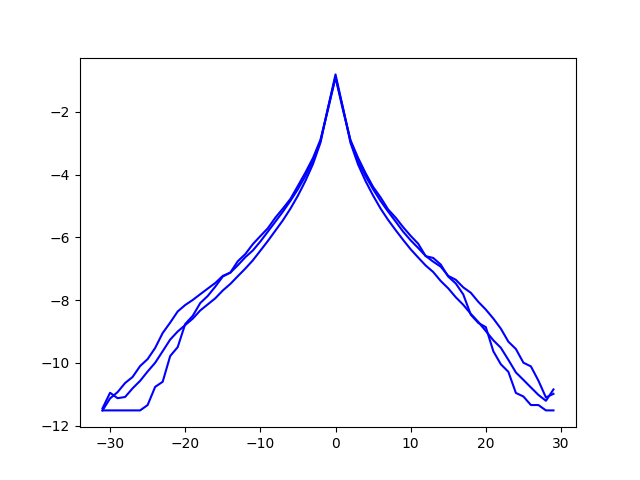
\includegraphics[scale=0.25]{pro1_result/downsampled_histogram/composed_log_setA.png}
    }
    \subfigure[Set B]{
        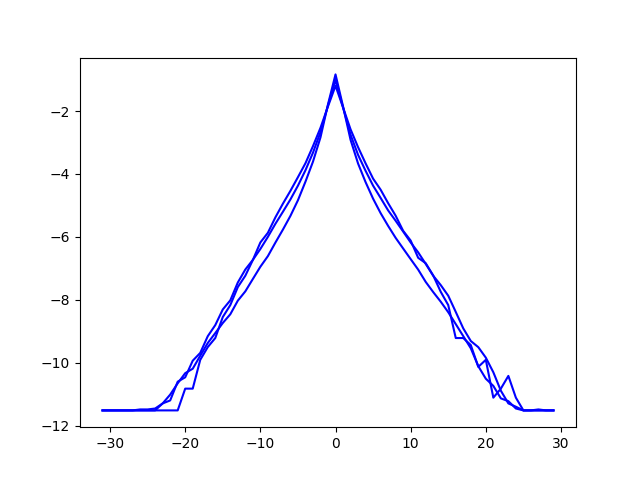
\includegraphics[scale=0.25]{pro1_result/downsampled_histogram/composed_log_setB.png}
    }
    \subfigure[Set C]{
        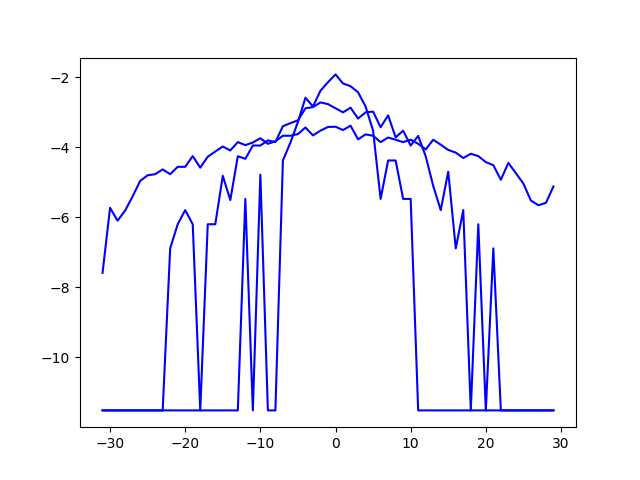
\includegraphics[scale=0.25]{pro1_result/downsampled_histogram/composed_log_setC.png}
    }
    \caption{log-histograms and downsamples}
\end{figure}

\end{enumerate}

\clearpage

\noindent{\bf Problem 2}. (Verify the 1/f power law observation in natural images, 3 points). \emph{Please read through this question description before you start. For this problem, please only consider set A.}

\noindent{Perform} a Fast Fourier Transform (FFT) on the grayscale image denoted as $I$. This operation will yield a Fourier image denoted as $\hat I(\xi, \eta)$, which is a complex-number matrix indexed by horizontal and vertical frequencies $(\xi, \eta)$. Subsequently, compute the amplitude (modulus) of each complex number, denoted as $A(\xi, \eta)$, and it can be calculated as follows: $A(\xi, \eta) = |\hat I(\xi, \eta)|$. Denote the frequency $f=\sqrt{\xi^2 + \eta^2}$, and to facilitate further analysis, convert the data to polar coordinates. In this coordinate system, calculate the total Fourier power, denoted as $A^2(f)$, for each frequency. To achieve this, discretize the values of $f$ and compute $A^2(f)$ averaged over the respective ring corresponding to each value of $f$. It is important to terminate the process when the circle reaches the boundary of the Fourier image.

\begin{enumerate}

\item Plot $\log A(f)$ against $\log f$. This should be close to a straight line for each image. Plot the curves for the 4 images in one figure for comparison. [Hint: First check the magnitude spectrum $\log |\hat I(\xi, \eta)|$, $|\hat I(0, 0)|$ typically is the largest component of the spectrum. The dc component is usually moved to the center of the frequency rectangle.]

\Answer See the Figure 7
\begin{figure}[h]
    \centering
    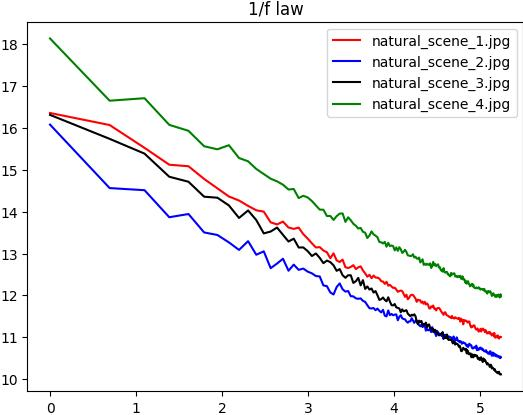
\includegraphics[scale=0.5]{pro2_result/f1_law.jpg}
    \caption{f1 law}
\end{figure}


\item Compute the integration (summation in discrete case) of $S(f_0) = \int_{\Omega} A^2(\xi, \eta) d\xi d\eta$ over the domain
 \[ \Omega(f_0) =\{(\xi, \eta): f_0 \leq \sqrt{\xi^2 + \eta^2} \leq 2f_0 \} \]
Plot $S(f_0)$ over $f_0$, the plot should fit to a horizontal line (with fluctuation) as $S(f_0)$ is supposed to be a constant over $f_0$.

\Answer See the Figure 8
\begin{figure}[h]
    \centering
    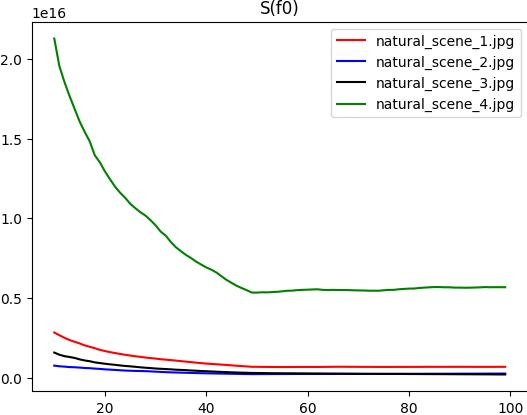
\includegraphics[scale=0.5]{pro2_result/S_f0.jpg}
    \caption{$S(f_0)$}
\end{figure}

\end{enumerate}

\clearpage

\noindent{\bf Problem 3}. (A 2D scale invariant world, 3 points). \emph{Please read through this question description before you start.}
 
\noindent{Let's} consider the simulation of a 2D world in which the images consist of only 1D line segments. Each line segment in an image can be characterized by its staring point $(x_i, y_i)$, orientation $\theta_i$, and length $r_i$. The line segments are independently distributed with uniform probability for their centers and orientations. The length of the line segments follows a probability distribution denoted as $p(r)$, which is proportional to $1/r^3$, representing a cubic power-law distribution. [Hint: How to sample $r$ from $p(r)$? Calculate the Cumulative Distribution function of $p(r)$, then draw a random number in [0,1].]

\begin{enumerate}
\item Simulate 1 image $I_1$ of size $1024 \times 1024$ pixels
with a total $N$ lines. (You need to truncate long lines and hide (discard) lines shorter than a pixel.)

\Answer See the Figure 9
\begin{figure}[h]
    \centering
    
\includegraphics[scale=0.25]{pro3_result/1024.png}
    \caption{$I_1$ with size of 1024$\times$1024}
\end{figure}

\item Simulate 2 new images $I_2$ and $I_3$ of size $512 \times 512$ and $256 \times 256$ pixels respectively. $I_2$ and $I_3$ are down-sampled version of $I_1$ and are generated by shortening the $N$ line segments in $I_1$ by $50\%$ and $25\%$ respectively (discard lines shorter than 1).

\Answer See the Figure 10
\begin{figure}[h]
    \centering
    \subfigure[512$\times$512]{
        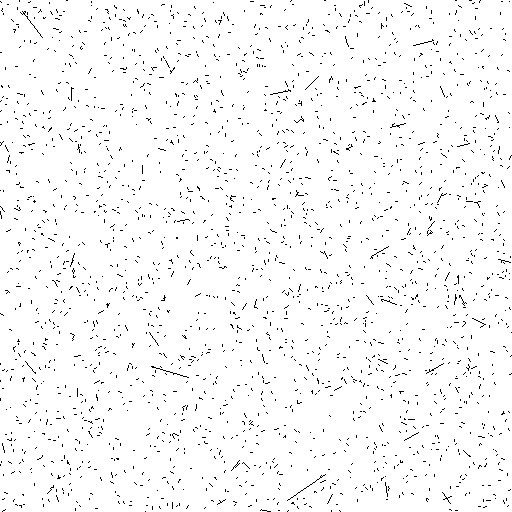
\includegraphics[scale=0.25]{pro3_result/512.png}
    }
    \subfigure[256$\times$256]{
        
\includegraphics[scale=0.5]{pro3_result/256.png}
    }
    \caption{$I_2$ with size of 512$\times$512 and $I_3$ with size of 256$\times$256}
\end{figure}

\item Crop 2 image patches of size $128 \times 128$ pixels randomly from each of the three images $I_1, I_2, I_3$ respectively. Plot these six images [draw the line segments in black on white background].

\Answer See the Figure 11
\begin{figure}[h]
    \centering
    \subfigure[crop from 1024]{
        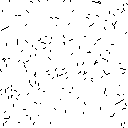
\includegraphics[scale=1]{pro3_result/crop/1024crop0.png}
    }
    \subfigure[crop from 512]{
        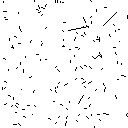
\includegraphics[scale=1]{pro3_result/crop/512crop0.png}
    }
    \subfigure[crop from 256]{
        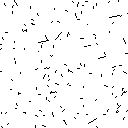
\includegraphics[scale=1]{pro3_result/crop/256crop0.png}
    }

    \subfigure[crop from 1024]{
        
\includegraphics[scale=1]{pro3_result/crop/1024crop1.png}
    }
    \subfigure[crop from 512]{
        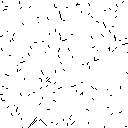
\includegraphics[scale=1]{pro3_result/crop/512crop1.png}
    }
    \subfigure[crop from 256]{
        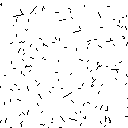
\includegraphics[scale=1]{pro3_result/crop/256crop1.png}
    }
    \caption{Images cropped from $I_1,I_2,I_3$}
\end{figure}
\end{enumerate}

If you did it right [Please try!], the 6 images must look the same (i.e., you should not be able to tell what scale the 6 images are cropped from). As a result, this 2D world is scale-invariant.

\end{document}
